\subsection*{Problema 38}

\textbf{Enunciado:} 
Calcular la integral indefinida:
\begin{align*}
I = \int \dfrac{x^5}{(x^3 + 1)(x^3 + 8)} \, dx
\end{align*}

\textbf{Solución:}
Siguiendo la indicación, realizamos el cambio de variable:
\begin{align*}
u &= x^3, \quad du = 3x^2 \, dx \\
\dfrac{du}{3} &= x^2 \, dx
\end{align*}

Reescribimos el integrando para hacer visible el término $x^2 \, dx$:
\begin{align*}
I &= \int \dfrac{x^3 \cdot x^2}{(x^3 + 1)(x^3 + 8)} \, dx \\
I &= \int \dfrac{u}{(u + 1)(u + 8)} \left(\dfrac{du}{3}\right) \\
I &= \dfrac{1}{3} \int \dfrac{u}{(u + 1)(u + 8)} \, du
\end{align*}

Aplicamos descomposición en fracciones parciales al integrando en la variable $u$:
\begin{align*}
\dfrac{u}{(u + 1)(u + 8)} &= \dfrac{A}{u + 1} + \dfrac{B}{u + 8}
\end{align*}

Multiplicando por el denominador común:
\begin{align*}
u &= A(u + 8) + B(u + 1)
\end{align*}

Evaluando para $u = -1$:
\begin{align*}
-1 &= A(-1 + 8) \implies 7A = -1 \implies A = -\dfrac{1}{7}
\end{align*}

Evaluando para $u = -8$:
\begin{align*}
-8 &= B(-8 + 1) \implies -7B = -8 \implies B = \dfrac{8}{7}
\end{align*}

Sustituimos las constantes en la integral:
\begin{align*}
I &= \dfrac{1}{3} \int \left( \dfrac{-1/7}{u + 1} + \dfrac{8/7}{u + 8} \right) du \\
I &= \dfrac{1}{21} \int \left( -\dfrac{1}{u + 1} + \dfrac{8}{u + 8} \right) du
\end{align*}

Integramos cada término respecto a $u$:
\begin{align*}
I &= \dfrac{1}{21} \left( -\ln|u + 1| + 8\ln|u + 8| \right) + C
\end{align*}

Regresando a la variable original $x$ mediante $u = x^3$:
\begin{align*}
I &= \dfrac{1}{21} \left( 8\ln|x^3 + 8| - \ln|x^3 + 1| \right) + C
\end{align*}

Por lo tanto, la solución general es:
\begin{align*}
I &= \dfrac{1}{21} \ln\left| \dfrac{(x^3 + 8)^8}{x^3 + 1} \right| + C
\end{align*}

\begin{figure}[H]
	\centering
	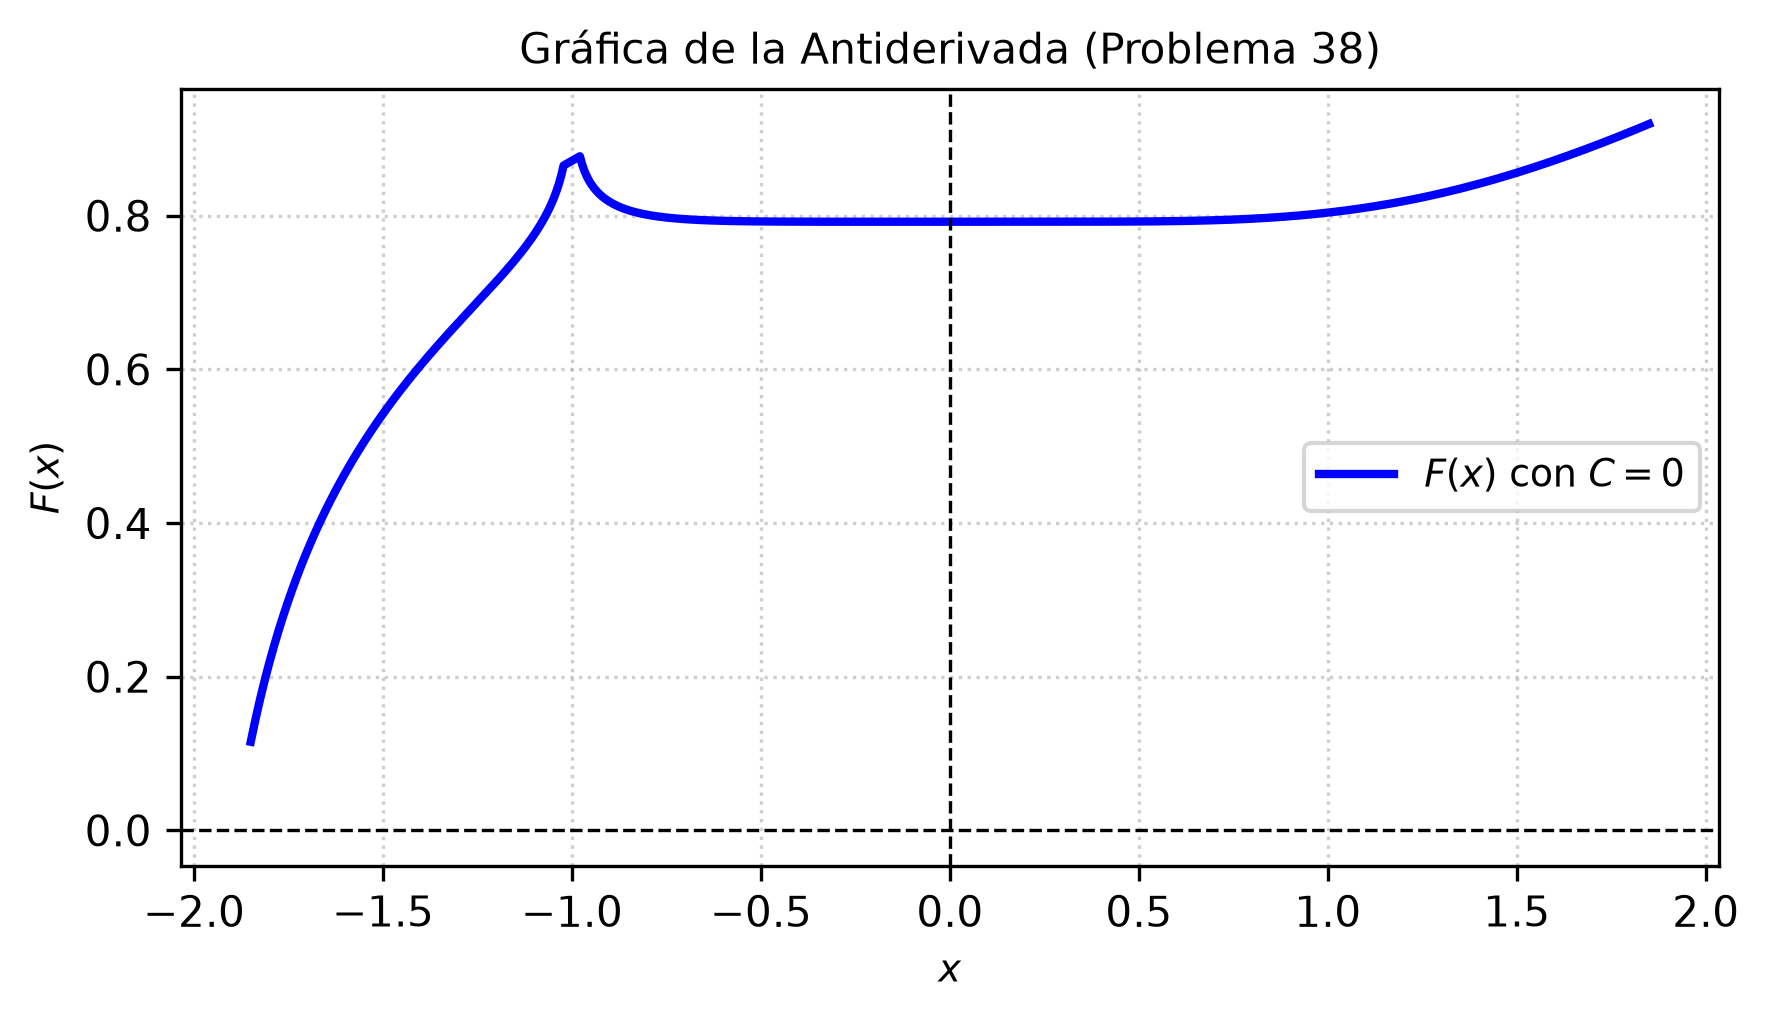
\includegraphics[width=\columnwidth]{semana_03/graficas/SEM03_P38_grafica.png}
	\caption{Representación gráfica de $f(x)$ y su antiderivada $F(x)$ evaluada para la constante de integración $C = 0$ (Problema 38).}
	\label{fig:problema38}
\end{figure}
